\documentclass{standalone}
\usepackage{tikz}
\begin{document}
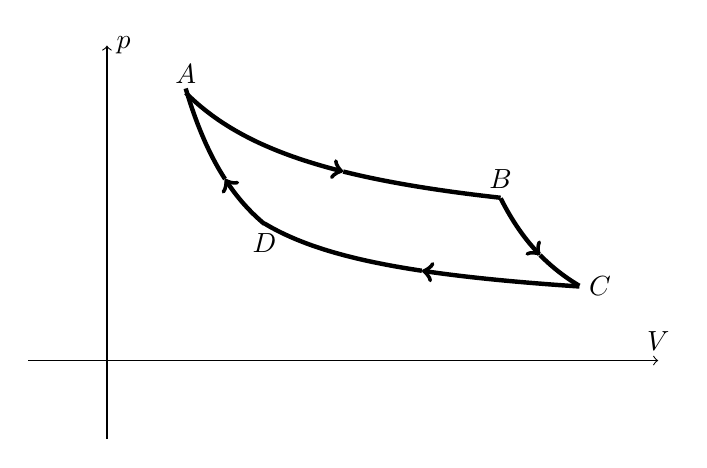
\begin{tikzpicture}[scale=2]

    \draw[->](-0.5,0)--(3.5,0)node[above]{$V$};
    \draw[->](0,-0.5)--(0,2)node[right]{$p$};

    \draw[->,ultra thick]plot[smooth, domain=0.5:1.5](\x,{0.7+1/(\x+0.5)});
    \draw[-,ultra thick]plot[smooth, domain=1.5:2.5](\x,{0.7+1/(\x+0.5)});
    
    \draw[->,ultra thick]plot[smooth, domain=2.5:2.75](\x,{0.03+1/(\x-1.5)^2});
    \draw[-,ultra thick]plot[smooth, domain=2.75:3](\x,{0.03+1/(\x-1.5)^2});

    \draw[-,ultra thick]plot[smooth, domain=1:2](\x,{0.27+0.6/(\x)});
    \draw[<-,ultra thick]plot[smooth, domain=2:3](\x,{0.27+0.6/(\x)});

    \draw[<-,ultra thick]plot[smooth, domain=0.75:1](\x,{0.31+1/(\x+0.34)^2});
    \draw[-,ultra thick]plot[smooth, domain=0.5:0.75](\x,{0.31+1/(\x+0.34)^2});


    \node[above]at(0.5,1.7){$A$};
    \node[above]at(2.5,1.03){$B$};
    \node[right]at(3,0.474){$C$};
    \node[below]at(1,0.87){$D$};
\end{tikzpicture}
\end{document}